\label{texfile:GWF}
A \mfus\ 3D groundwater flow (GWF) domain can be generated from the template using the
instruction \textsf{generate layered gwf domain}, with the option of defining the \mf\ cell control volumes using template mesh element (mesh-centred  control volume) or node (node-centred control volume) locations.  , as shown in Figure~\ref{fig:ControlVolumes} for a triangular-element template mesh.
    \vspace{.2in} \\
   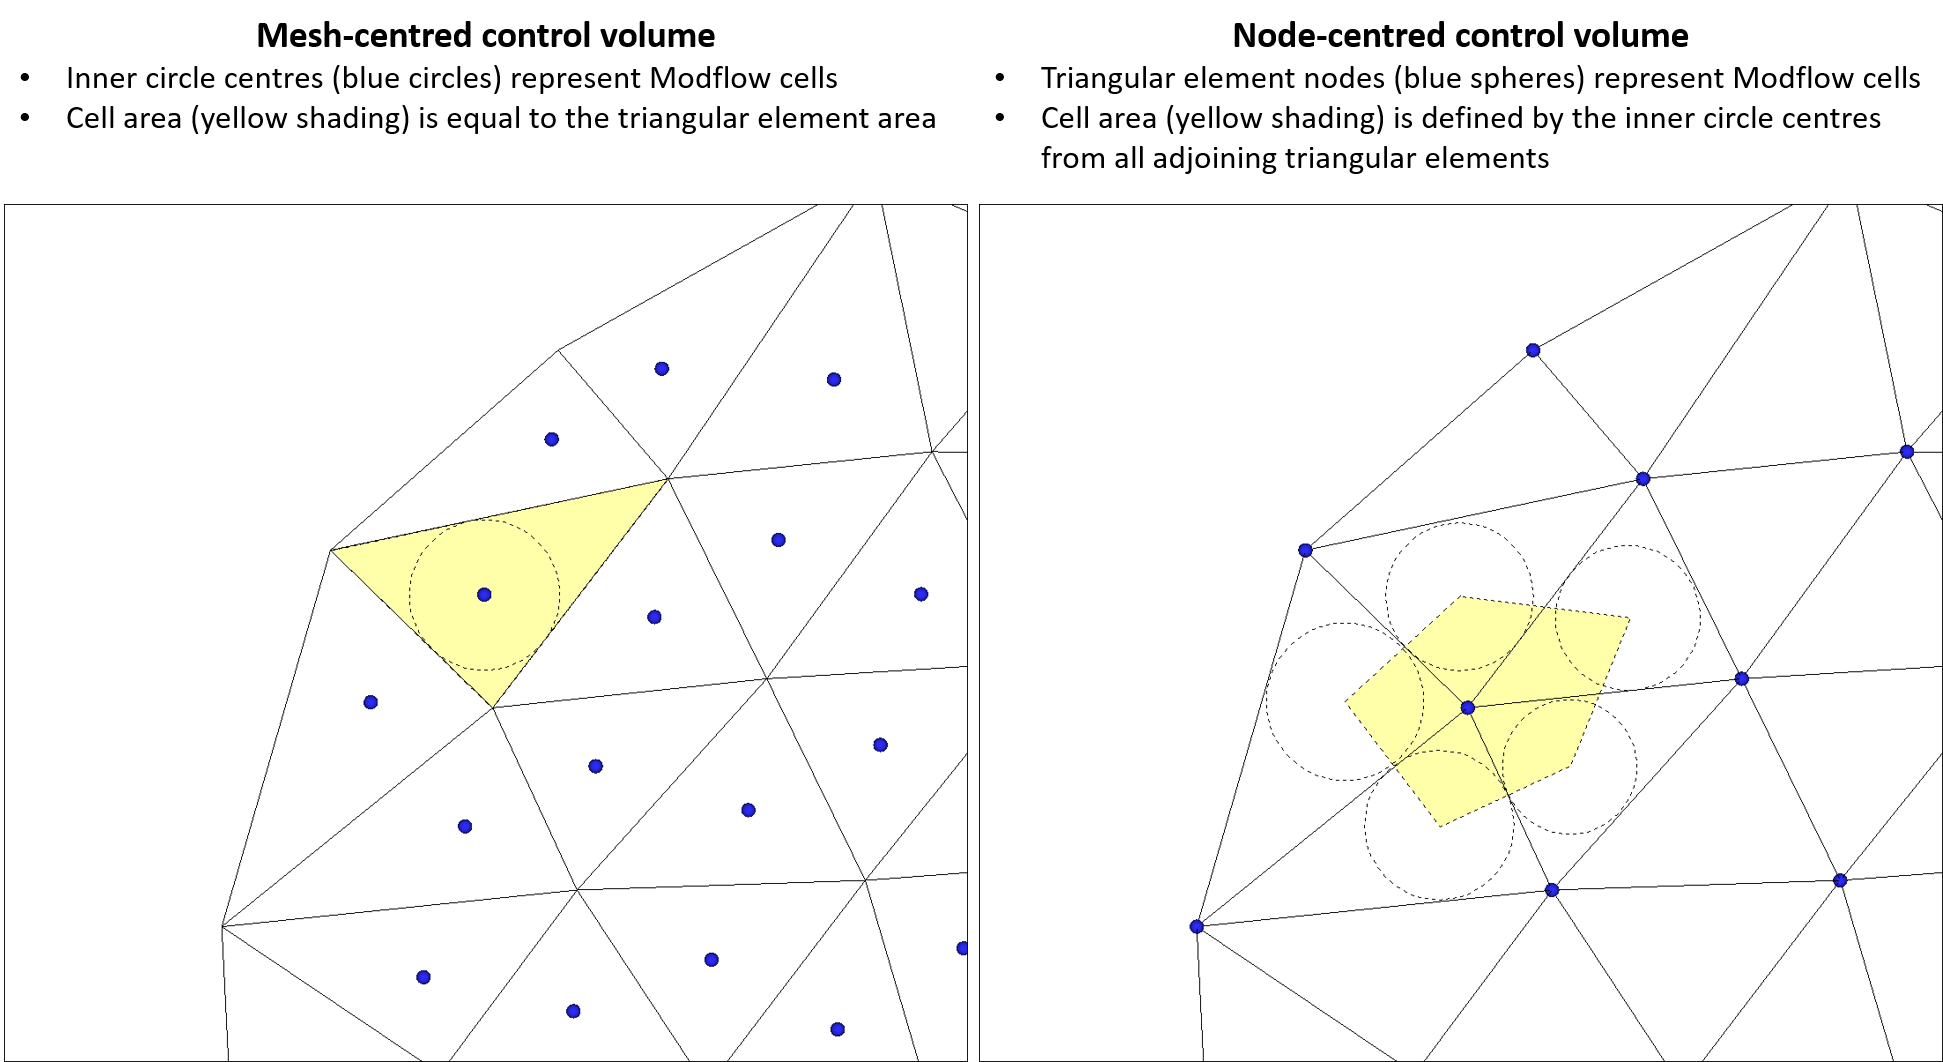
\includegraphics[width=0.9\textwidth]{ControlVolume}
    \vspace{.2in} \\
Note the following:
\begin{figure}
     \caption{Modflow cell control volume types defined from a triangular-element mesh.  On the left is a mesh-centred control volume, on the right a node-centred control volume.}
    \label{fig:ControlVolumes}
\end{figure}
By default, the mesh-centred  control volume approach is used. If you would like to use the node-centred control volume approach instead, the first entry in the \texttt{build modflow usg} subtask should be:
\begin{verbatim}
    nodal control volumes
\end{verbatim}





, as shown in this example:
\begin{verbatim}
    generate layered gwf domain

        top elevation
            elevation constant
            100.0
        end top elevation

        new layer
            layer name
            Top layer

            uniform sublayering
            100

            elevation constant
            0.0
        end new layer

    end generate layered gwf domain
\end{verbatim}
The \textsf{generate layered gwf domain} instruction is a subtask so it has a corresponding \textsf{end generate layered gwf domain} instruction.  The GWF domain is generated from the top layer down, and the first instruction, \textsf{top elevation}, defines the ground surface elevation at the layer of elements in the TECPLOT\_GWF mesh. It must begin with a \textsf{top elevation} instruction and at least one \textsf{new layer} instruction. Not shown in this example is an optional additional instruction, \textsf{zone by template}.

 There are options for defining the top elevation:
\begin{description}
  \item[elevation constant] The value is assigned to all nodes in the top sheet of the TECPLOT\_GWF mesh.
  \item[elevation from gb file] The file
  \item[elevation from ascii file] The file
  \item[elevation from xz pairs] The list

\end{description}
